% !TEX encoding = UTF-8
% !TEX TS-program = pdflatex
% !TEX root = ../Tesi.tex
% !TEX spellcheck = en-EN

%************************************************
\chapter{Blast Furnace}
\label{cap:blastfurnace}
%************************************************

\info{incomplete}

The raceway, a critical portion of the blast furnace (Fig.
\ref{fig:068racewaylayout}), was investigated.
We performed a limited number of simulations of this volume to investigate the
effect of the variation of input velocity.\\
The results presented in Fig. \ref{fig:068racewaylayout}, Fig.
\ref{fig:225racewayu}, Fig. \ref{fig:238racewayus}, and Fig.
\ref{fig:239racewayvf} were later compared with the literature data from
\citet{RefWorks:208}.

\begin{figure}[!htb]
\centering
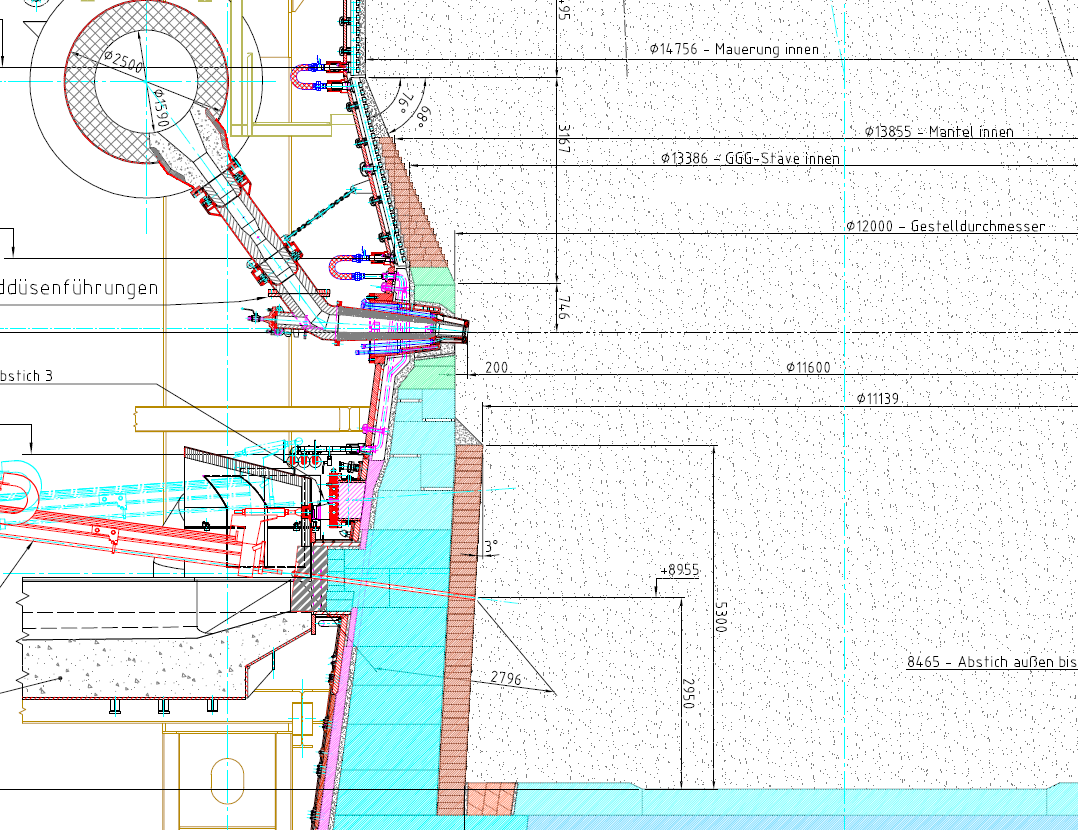
\includegraphics[width=.80\columnwidth]{images/068racewaylayout}
\caption[Blast furnace section layout]{Blast furnace section layout (Voestalpine Stahl GmbH).}
\label{fig:068racewaylayout}
\end{figure}

\newpage

\section{Results}
\label{sec:resultsbf}

We considered a portion of the blast furnace center on a single tuyere (x = 0.0,
y = 0.0, z = 0.0).
The hot gases are injected along the x direction, and z represents the vertical
direction.
The domain is developed as follow:
\begin{itemize}
  \item{$0.0 < x < 2.0 m$,}
  \item{$-0.75 < y_1 < -0.6 m$, $-0.6 < y_2 < 0.6 m$,}
  \item{$-1.0 < z < 1.5 m$.} 
\end{itemize}

The change of sliding and rolling friction coefficients bear no effect on the
velocity of the gases. 
Their exit path is clearly accessible and the same kinetic energy, and thus velocity, was
dissipated to displace particles, see Fig. \ref{fig:225racewayu}.
Instead, the increase of the inlet velocity from 100 m/s to 200 m/s clearly
increments the raceway area by 50\%.\\
However, the particles velocity is clearly, and logically, higher for low
friction particles. They could be moved by the flow more easily compared to high
friction particles, see Fig. \ref{fig:238racewayus}.
Similarly, the increase of the inlet velocity from 100 m/s to 200 m/s clearly
increments the fast particle area by 50\%.\\
Concerning the void fraction, low friction allowed a better compaction of the
particles in the top volume, see Fig. \ref{fig:239racewayvf}.
Consequently, the gases need to travel less to reach the top empty volume.
The volume interested by an higher void fraction as effect of the raceway is
thus smaller.\\
If we combine the information from the previous images we obtain Fig.
\ref{fig:265racewaysummary}.
As we can see, the only relevant effect for the height and width of the raceway
area is due to the increase in the inlet velocity. 
We also investigated the height of the ``chimney'', an area over the
raceway, where the fluid and particles velocities are still high.
As can be seen in Fig. \ref{fig:264DeletedParticles}, this value increases
proportionally to the increase of the friction coefficients, but naturally
reaches a maximum with the fast inlet velocity simulation.
The kinetic energy of the fluid could not be dissipated for moving particles
already in the proximity area of the tuyere.
Consequently, it has remained high in a larger area.\\
Further, the low friction particles tend to flow more easily in the raceway volume. 
Thus, the delete atoms command is more effective than in the high friction case,
because more particles reach the deletion area.
Increasing the inlet velocity allows even more particles to reach the area,
displaced by the fast fluid.
\begin{figure}[!htb]
\centering
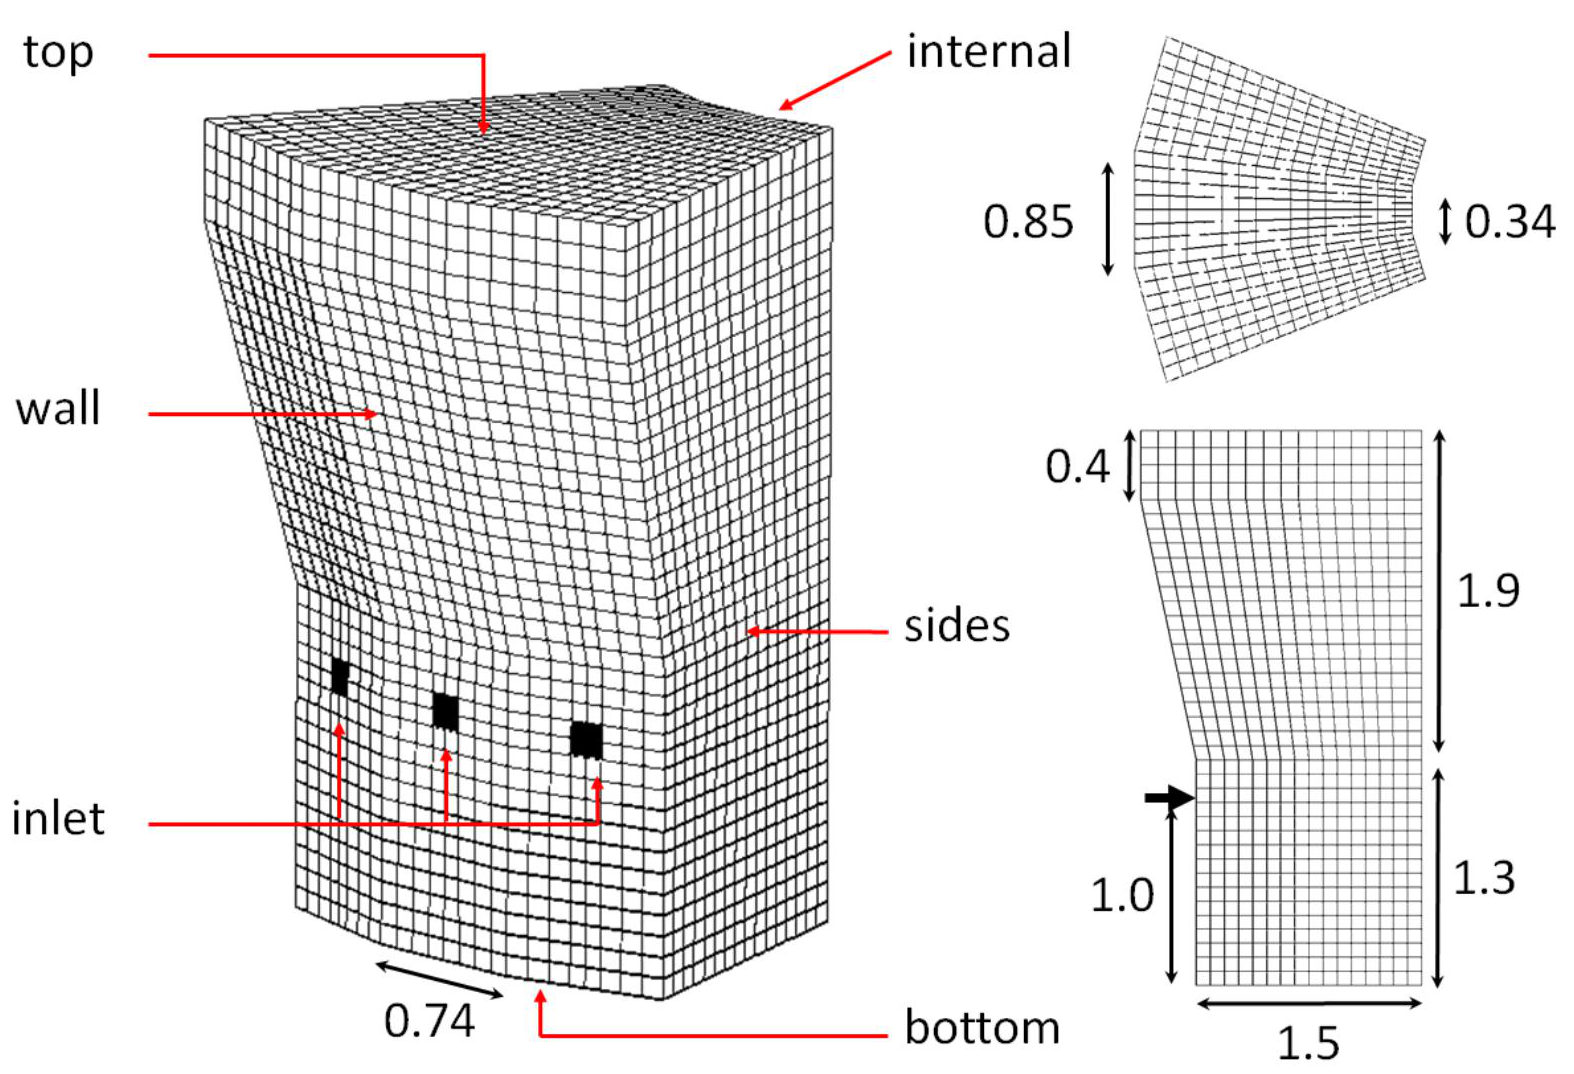
\includegraphics[width=.80\columnwidth]{images/273layoutbf}
\caption[Blast furnace simulation layout]{Blast furnace simulation layout \cite{RefWorks:208}.}
\label{fig:273layoutbf}
\end{figure}

\begin{figure}[htbp]
\centering 
  \subfloat[\acs{mus} = 0.1, $u_{lim}$ = 4 m/s]
  {
	  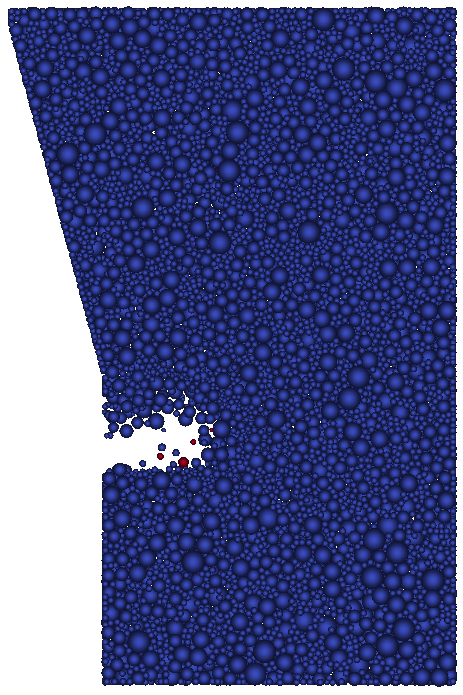
\includegraphics[width=.21\columnwidth]{images/296ver_slice_4mslf}
	  \label{fig:296ver_slice_4mslf}
  }
  \quad
    \subfloat[\acs{mus} = 0.1, $u_{lim}$ = 0.1 m/s]
    {
	  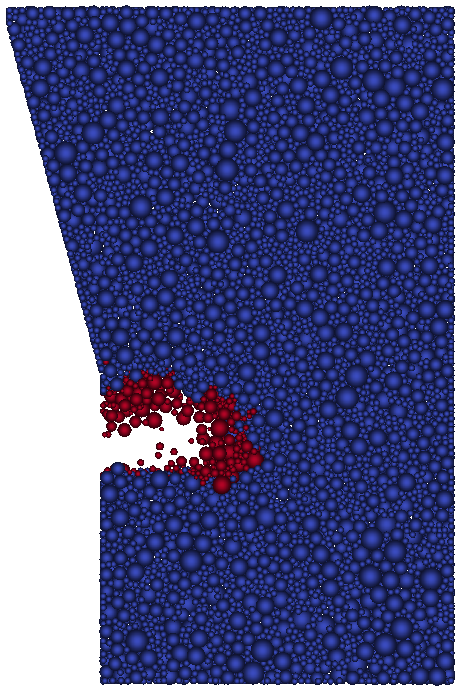
\includegraphics[width=.21\columnwidth]{images/295ver_slice_01mslf}
	  \label{fig:295ver_slice_01mslf}
  }
  \quad
    \subfloat[\acs{mus} = 0.1, $u_{lim}$ = 0.01 m/s]
    {
	  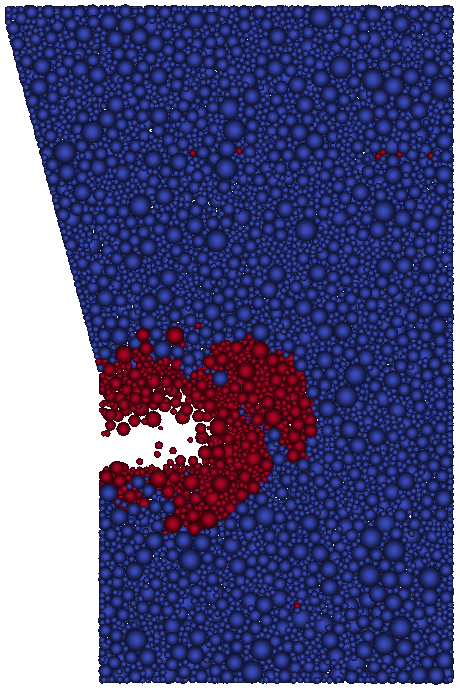
\includegraphics[width=.21\columnwidth]{images/294ver_slice_001mslf}
	  \label{fig:294ver_slice_001mslf}
  }
  \quad
  \subfloat[\acs{mus} = 0.1, $u_{lim}$ = 0.003 m/s]
  {
	  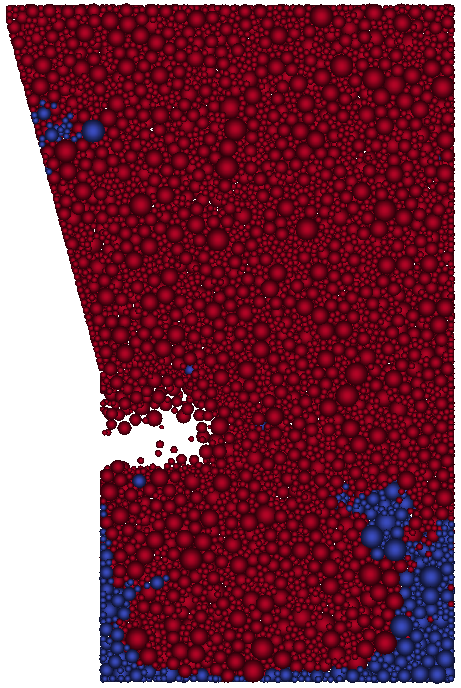
\includegraphics[width=.21\columnwidth]{images/293ver_slice_0003mslf}
	  \label{fig:293ver_slice_0003mslf}
  }
  \\
  \subfloat[\acs{mus} = 0.9, $u_{lim}$ = 4 m/s]
  {
	  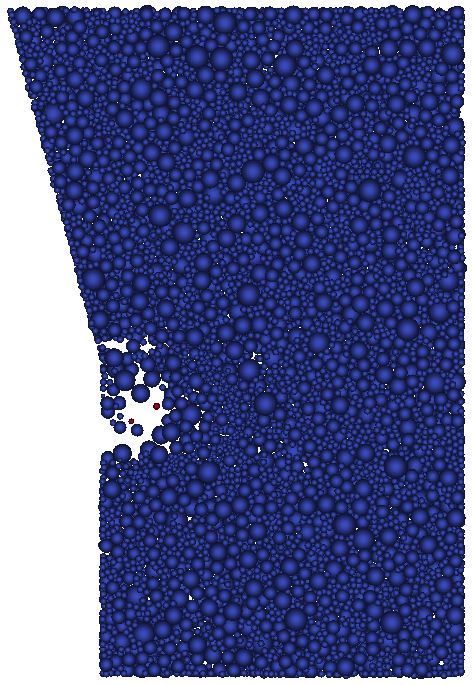
\includegraphics[width=.21\columnwidth]{images/266ver_slice_4mshf}
	  \label{fig:266ver_slice_4mshf}
  }
  \quad
    \subfloat[\acs{mus} = 0.9, $u_{lim}$ = 0.1 m/s]
    {
	  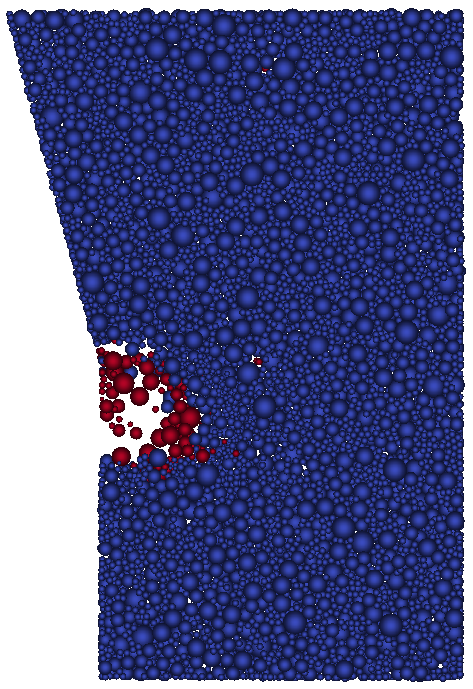
\includegraphics[width=.21\columnwidth]{images/267ver_slice_01mshf}
	  \label{fig:267ver_slice_01mshf}
  }
  \quad
    \subfloat[\acs{mus} = 0.9, $u_{lim}$ = 0.01 m/s]
    {
	  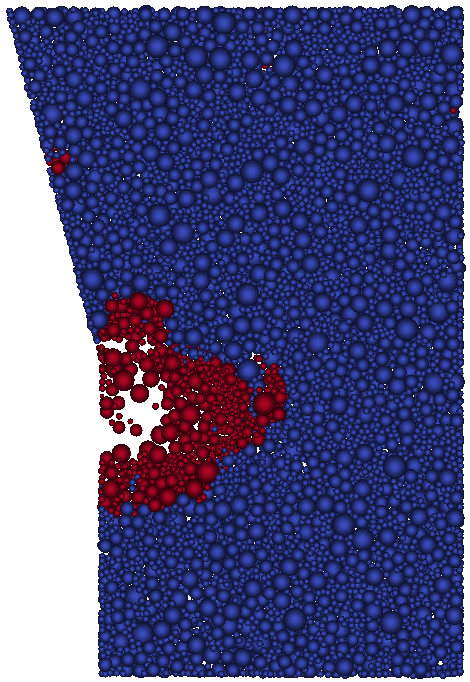
\includegraphics[width=.21\columnwidth]{images/268ver_slice_001mshf}
	  \label{fig:268ver_slice_001mshf}
  }
  \quad
  \subfloat[\acs{mus} = 0.9, $u_{lim}$ = 0.003 m/s]
  {
	  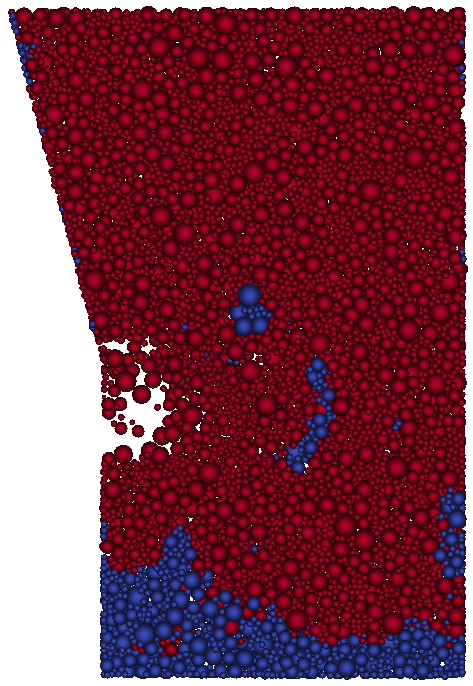
\includegraphics[width=.21\columnwidth]{images/269ver_slice_0003mshf}
	  \label{fig:269ver_slice_0003mshf}
  }
  \\  
  \caption[Vertical slice of particle velocity 2]{Vertical slice of particle
  velocity 2. Red particles are faster than the $u_{lim}$.}
  \label{fig:298verticalslicelf}
\end{figure}
\begin{figure}[htbp]
\centering 
  \subfloat[\acs{mus} = 0.1, \acs{mur} = 0.4, $v_{inlet}$ = 100 m/s .]
  {
	  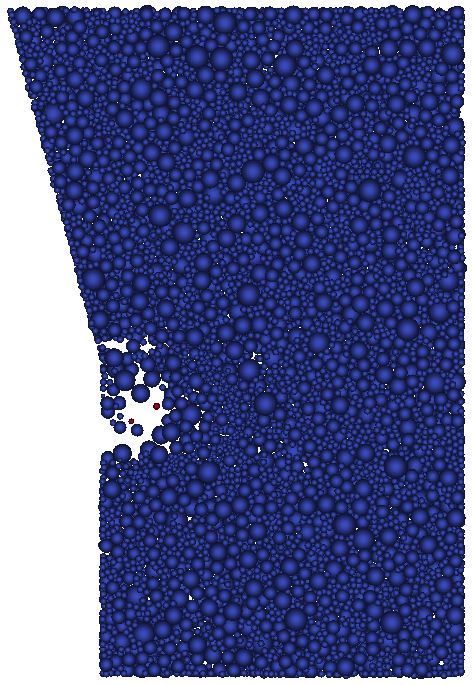
\includegraphics[width=.21\columnwidth]{images/266ver_slice_4mshf}
	  \label{fig:266ver_slice_4mshf}
  }
  \quad
    \subfloat[\acs{mus} = 0.5, \acs{mur} = 0.4, $v_{inlet}$ = 100 m/s .]
    {
	  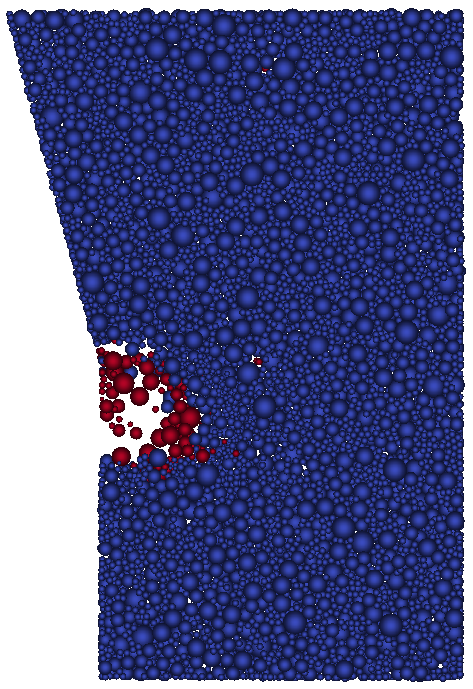
\includegraphics[width=.21\columnwidth]{images/267ver_slice_01mshf}
	  \label{fig:267ver_slice_01mshf}
  }
  \quad
    \subfloat[\acs{mus} = 0.9, \acs{mur} = 0.4, $v_{inlet}$ = 100 m/s .]
    {
	  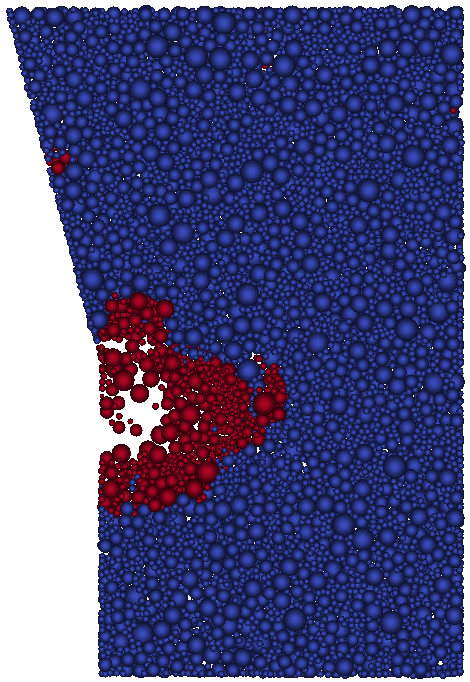
\includegraphics[width=.21\columnwidth]{images/268ver_slice_001mshf}
	  \label{fig:268ver_slice_001mshf}
  }
  \quad
  \subfloat[\acs{mus} = 0.1, \acs{mur} = 0.4, $v_{inlet}$ = 200 m/s .]
  {
	  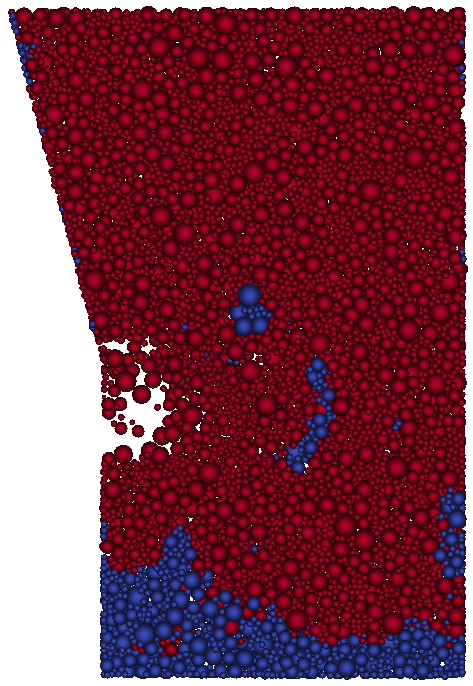
\includegraphics[width=.21\columnwidth]{images/269ver_slice_0003mshf}
	  \label{fig:269ver_slice_0003mshf}
  }
  \\
  \caption{282verticalslicehf.tex.}
  \label{fig:282verticalslicehf}
\end{figure}
\begin{figure}[htbp]
\centering 
  \subfloat[\acs{mus} = 0.1, spatial average.]
  {
	  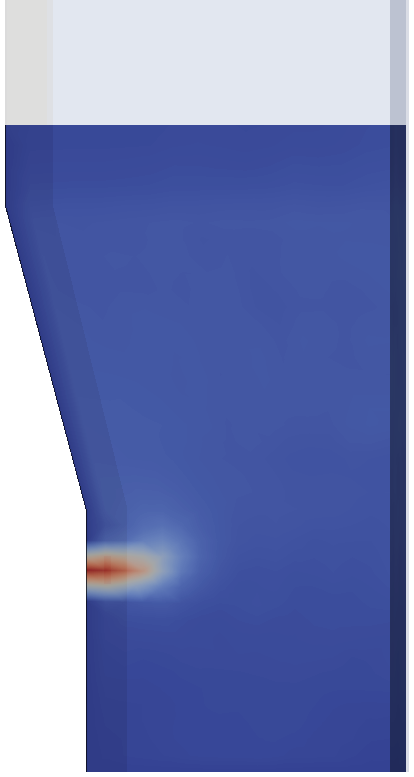
\includegraphics[width=.21\columnwidth]{images/288u_average_lf_stat}
	  \label{fig:288u_average_lf_stat}
  }
  \quad
    \subfloat[\acs{mus} = 0.1, velocity vectors.]
    {
	  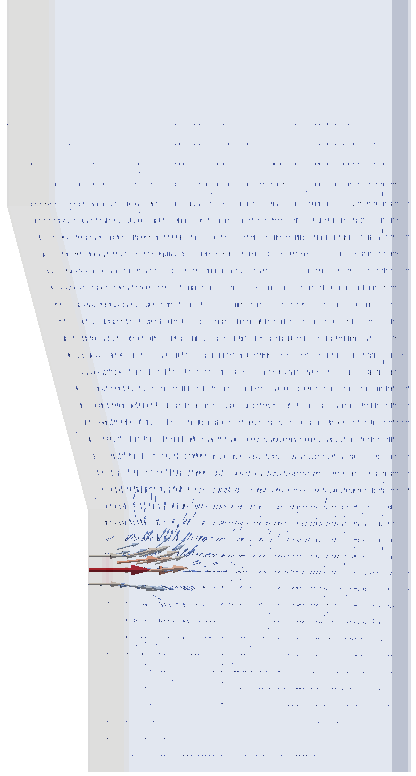
\includegraphics[width=.21\columnwidth]{images/287u_average_lf_arrow}
	  \label{fig:287u_average_lf_arrow}
  }
  \quad
    \subfloat[\acs{mus} = 0.1, stream lines.]
    {
	  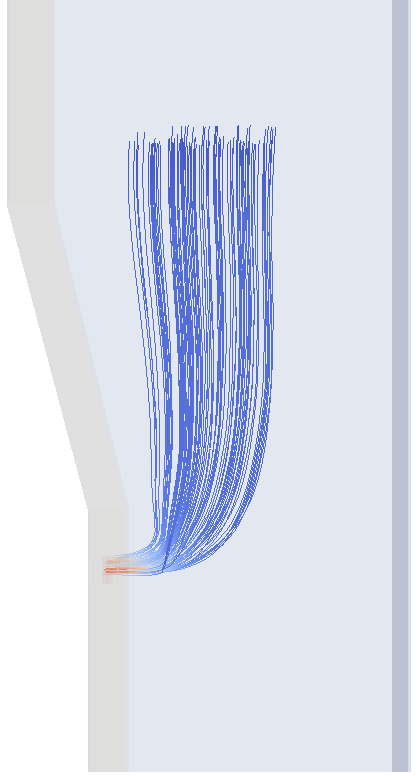
\includegraphics[width=.21\columnwidth]{images/289u_average_lf_stream}
	  \label{fig:289u_average_lf_stream}
  }
  \quad
  \subfloat[Legend.]
  {
	  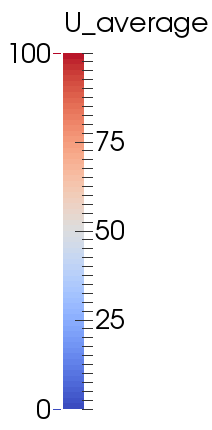
\includegraphics[width=.21\columnwidth]{images/274u_average_legend}
	  \label{fig:274u_average_legend}
  }
  \\
  \subfloat[\acs{mus} = 0.9, spatial average.]
  {
	  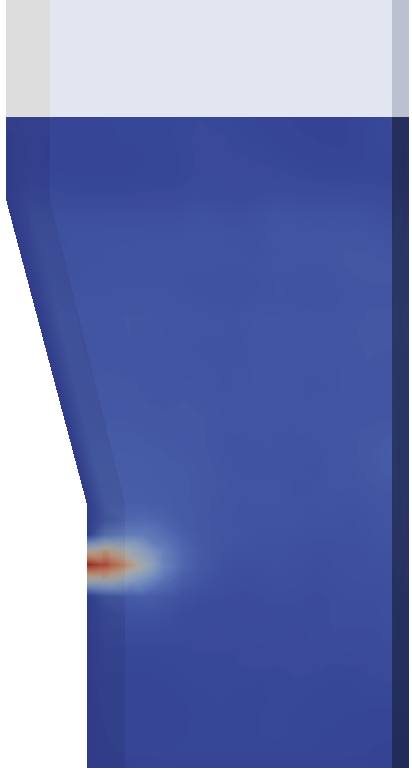
\includegraphics[width=.21\columnwidth]{images/276u_average_hf_stat}
	  \label{fig:276u_average_hf_stat}
  }
  \quad
    \subfloat[\acs{mus} = 0.9, velocity vectors.]
    {
	  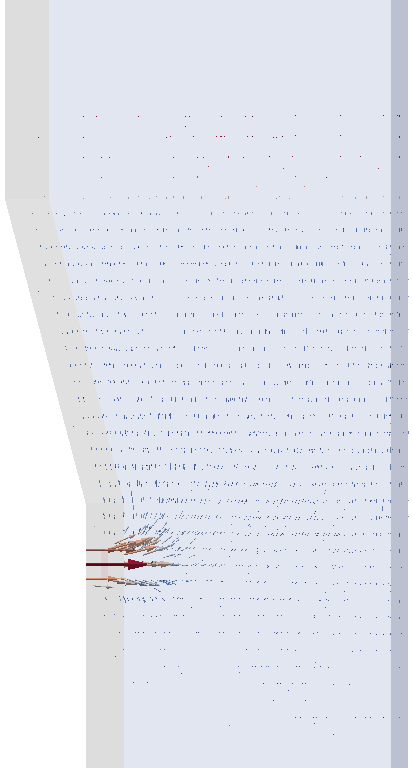
\includegraphics[width=.21\columnwidth]{images/275u_average_arrow}
	  \label{fig:275u_average_arrow}
  }
  \quad
    \subfloat[\acs{mus} = 0.9, stream lines.]
    {
	  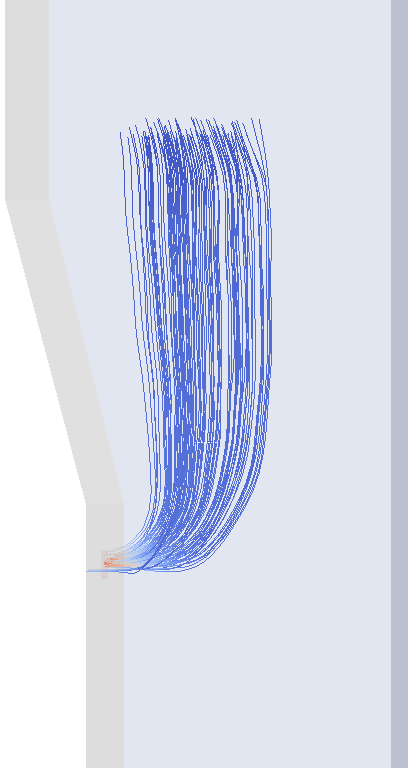
\includegraphics[width=.21\columnwidth]{images/277u_average_hf_stream}
	  \label{fig:277u_average_hf_stream}
  }
  \quad
  \subfloat[Legend.]
  {
	  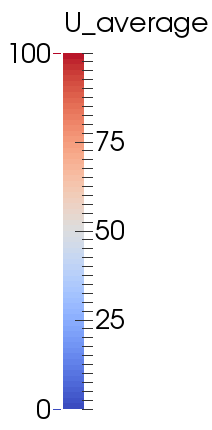
\includegraphics[width=.21\columnwidth]{images/274u_average_legend}
	  \label{fig:274u_average_legend}
  }
  \\  
  \caption[Vertical slice of fluid velocity]{Vertical slice of fluid velocity.}
  \label{fig:299u_average_lf}
\end{figure}
\begin{figure}[htbp]
\centering 
  \subfloat[\acs{mus} = 0.1, \acs{mur} = 0.4, $v_{inlet}$ = 100 m/s .]
  {
	  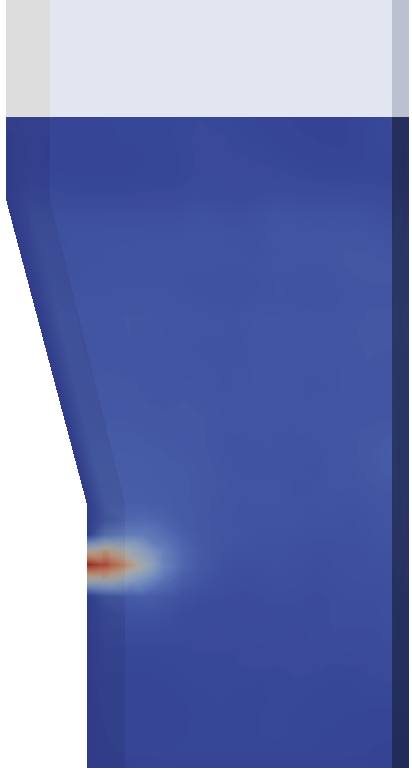
\includegraphics[width=.21\columnwidth]{images/276u_average_hf_stat}
	  \label{fig:276u_average_hf_stat}
  }
  \quad
    \subfloat[\acs{mus} = 0.5, \acs{mur} = 0.4, $v_{inlet}$ = 100 m/s .]
    {
	  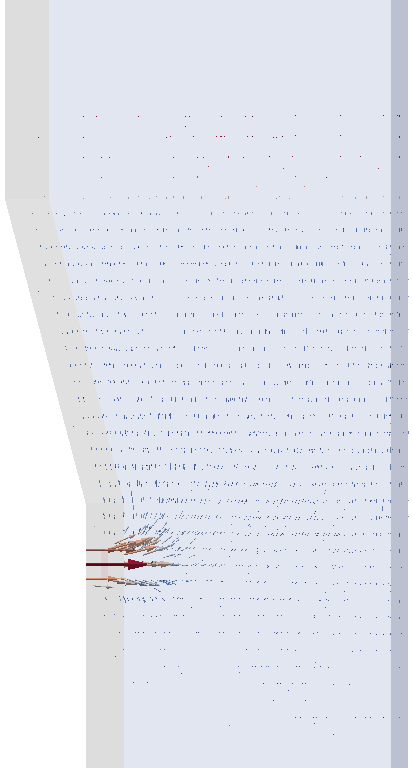
\includegraphics[width=.21\columnwidth]{images/275u_average_arrow}
	  \label{fig:275u_average_arrow}
  }
  \quad
    \subfloat[\acs{mus} = 0.9, \acs{mur} = 0.4, $v_{inlet}$ = 100 m/s .]
    {
	  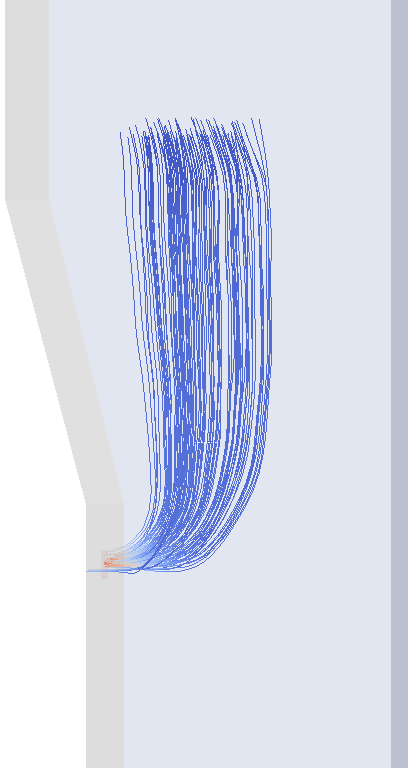
\includegraphics[width=.21\columnwidth]{images/277u_average_hf_stream}
	  \label{fig:277u_average_hf_stream}
  }
  \quad
  \subfloat[\acs{mus} = 0.1, \acs{mur} = 0.4, $v_{inlet}$ = 200 m/s .]
  {
	  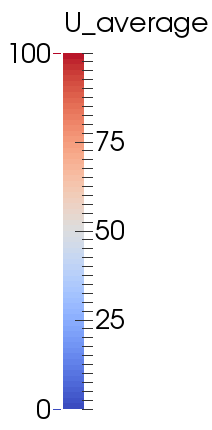
\includegraphics[width=.21\columnwidth]{images/274u_average_legend}
	  \label{fig:274u_average_legend}
  }
  \\
  \caption{283u_average_hf .}
  \label{fig:283u_average_hf}
\end{figure}
\begin{figure}[htbp]
\centering 
  \subfloat[\acs{mus} = 0.1, \acs{mur} = 0.4, $v_{inlet}$ = 100 m/s .]
  {
	  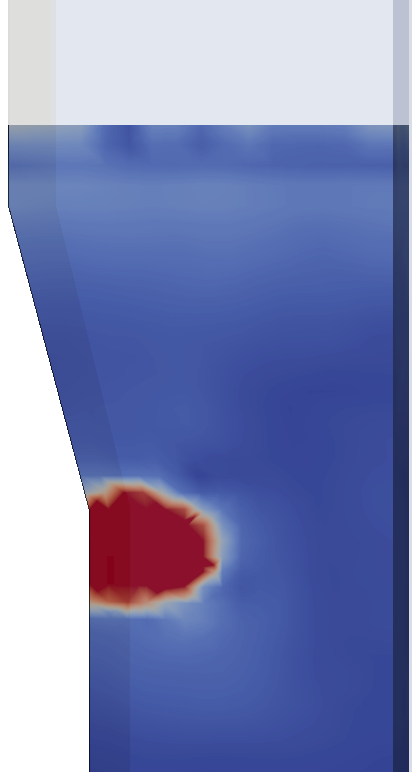
\includegraphics[width=.22\columnwidth]{images/291us_average_lf_stat}
	  \label{fig:291us_average_lf_stat}
  }
  \quad
    \subfloat[\acs{mus} = 0.5, \acs{mur} = 0.4, $v_{inlet}$ = 100 m/s .]
    {
	  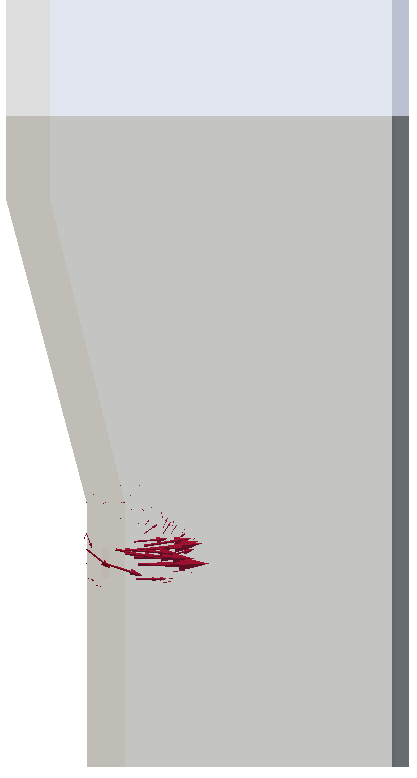
\includegraphics[width=.21\columnwidth]{images/290us_average_lf_arrow}
	  \label{fig:290us_average_lf_arrow}
  }
  \quad
    \subfloat[\acs{mus} = 0.9, \acs{mur} = 0.4, $v_{inlet}$ = 100 m/s .]
    {
	  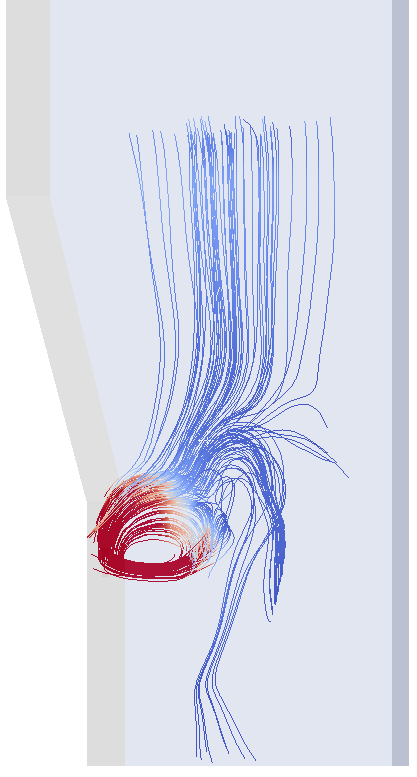
\includegraphics[width=.21\columnwidth]{images/292us_average_lf_stream}
	  \label{fig:292us_average_lf_stream}
  }
  \quad
  \subfloat[\acs{mus} = 0.1, \acs{mur} = 0.4, $v_{inlet}$ = 200 m/s .]
  {
	  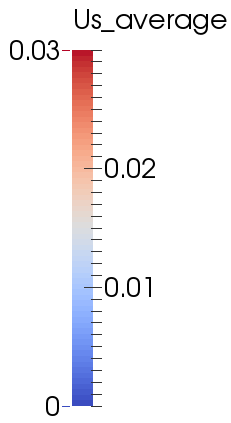
\includegraphics[width=.21\columnwidth]{images/278us_average_hf_legend}
	  \label{fig:278us_average_hf_legend}
  }
  \\
  \caption{300us_average_lf .}
  \label{fig:300us_average_lf}
\end{figure}
\begin{figure}[htbp]
\centering 
  \subfloat[\acs{mus} = 0.1, \acs{mur} = 0.4, $v_{inlet}$ = 100 m/s .]
  {
	  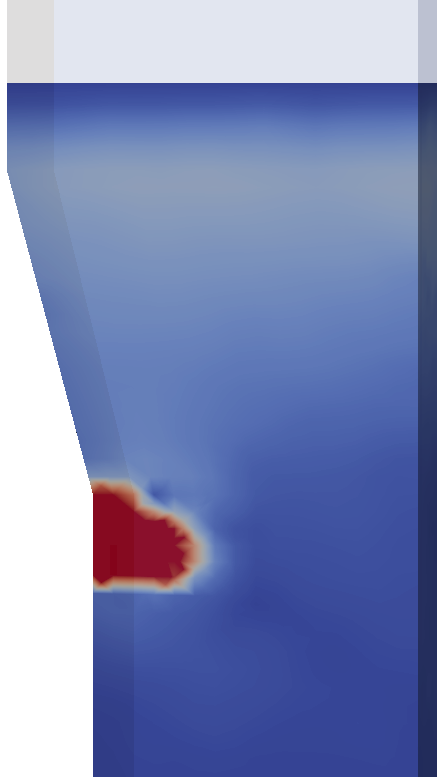
\includegraphics[width=.22\columnwidth]{images/280us_average_hf_stat}
	  \label{fig:280us_average_hf_stat}
  }
  \quad
    \subfloat[\acs{mus} = 0.5, \acs{mur} = 0.4, $v_{inlet}$ = 100 m/s .]
    {
	  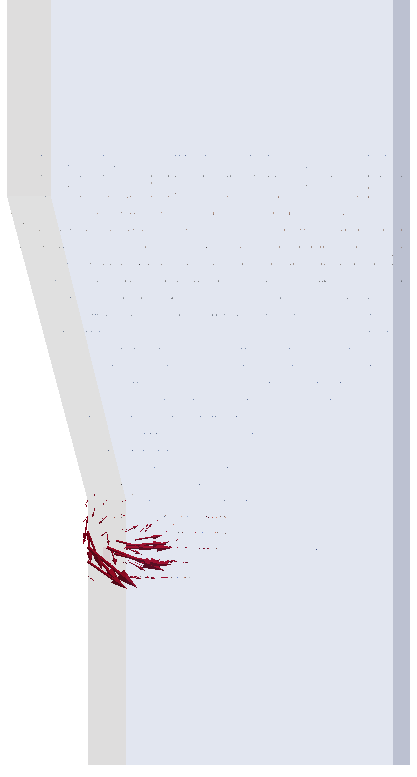
\includegraphics[width=.21\columnwidth]{images/279us_average_hf_arrow}
	  \label{fig:279us_average_hf_arrow}
  }
  \quad
    \subfloat[\acs{mus} = 0.9, \acs{mur} = 0.4, $v_{inlet}$ = 100 m/s .]
    {
	  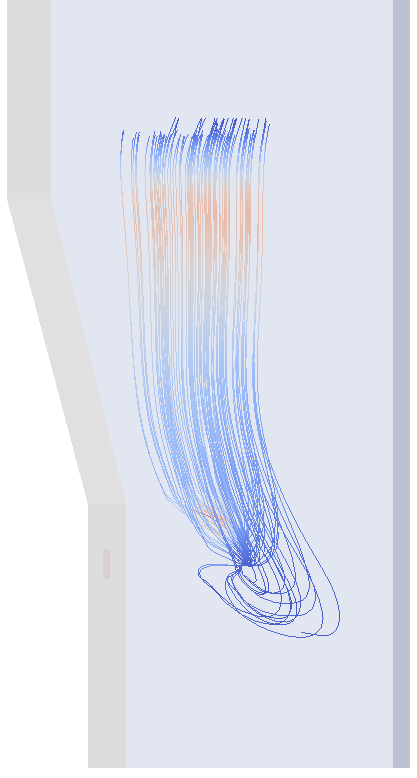
\includegraphics[width=.21\columnwidth]{images/281us_average_hf_stream}
	  \label{fig:281us_average_hf_stream}
  }
  \quad
  \subfloat[\acs{mus} = 0.1, \acs{mur} = 0.4, $v_{inlet}$ = 200 m/s .]
  {
	  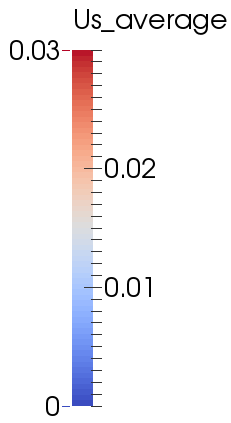
\includegraphics[width=.21\columnwidth]{images/278us_average_hf_legend}
	  \label{fig:278us_average_hf_legend}
  }
  \\
  \caption{284us_average_hf .}
  \label{fig:284us_average_hf}
\end{figure}
\begin{figure}[htbp]
\centering 
  \subfloat[\acs{mus} = 0.1 .]
  {
	  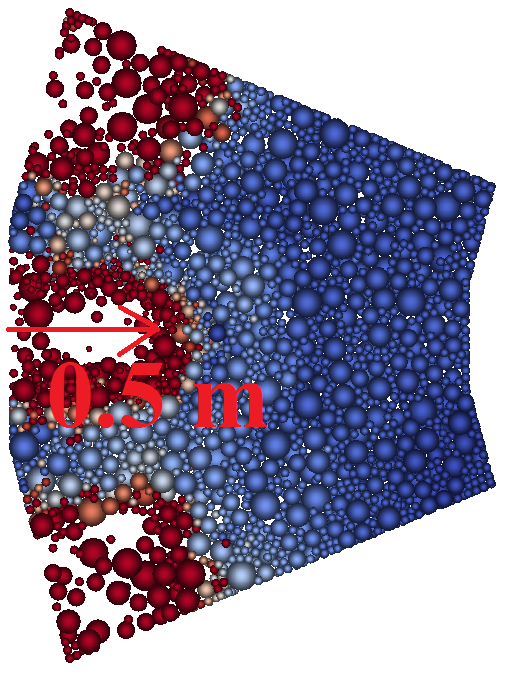
\includegraphics[width=.28\columnwidth]{images/285hor_slice_01mslf}
	  \label{fig:285hor_slice_01mslf}
  }
  \quad
    \subfloat[\acs{mus} = 0.9 .]
    {
	  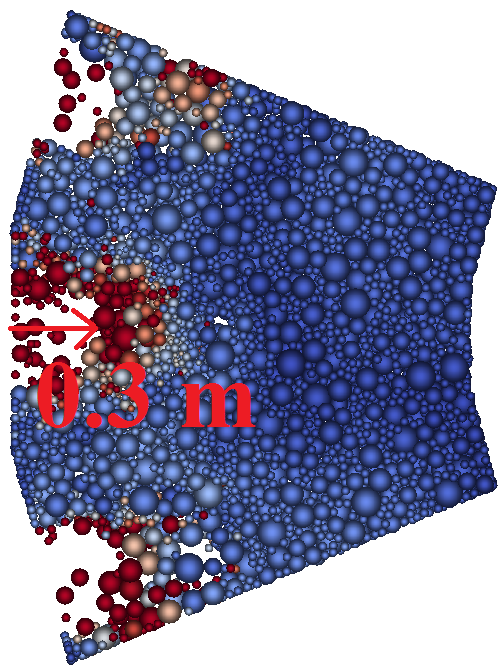
\includegraphics[width=.27\columnwidth]{images/271hor_slice_01mshf}
	  \label{fig:271hor_slice_01mshf}
  }
  \quad
    \subfloat[Legend and slice position.]
    {
	  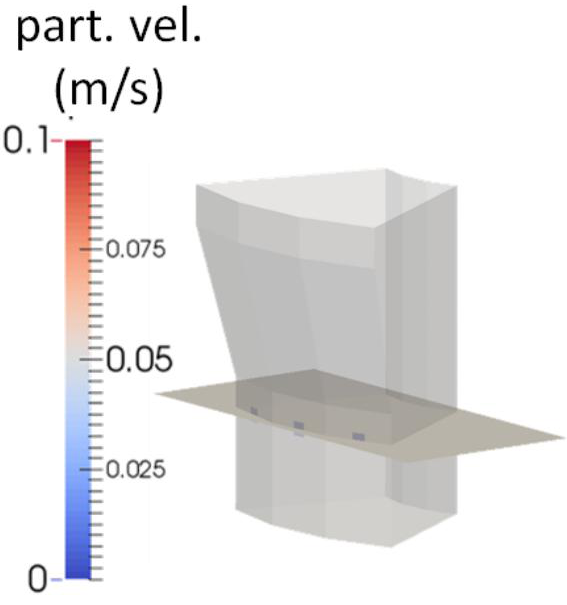
\includegraphics[width=.34\columnwidth]{images/272slice}
	  \label{fig:272slice}
  }
  \\
  \caption{Raceway penetration depth on the horizontal.}
  \label{fig:286hor_slice_01ms}
\end{figure}
% \begin{sidewaysfigure}[htbp]
\centering 
  \subfloat[Low friction, average velocity.]
  {
	  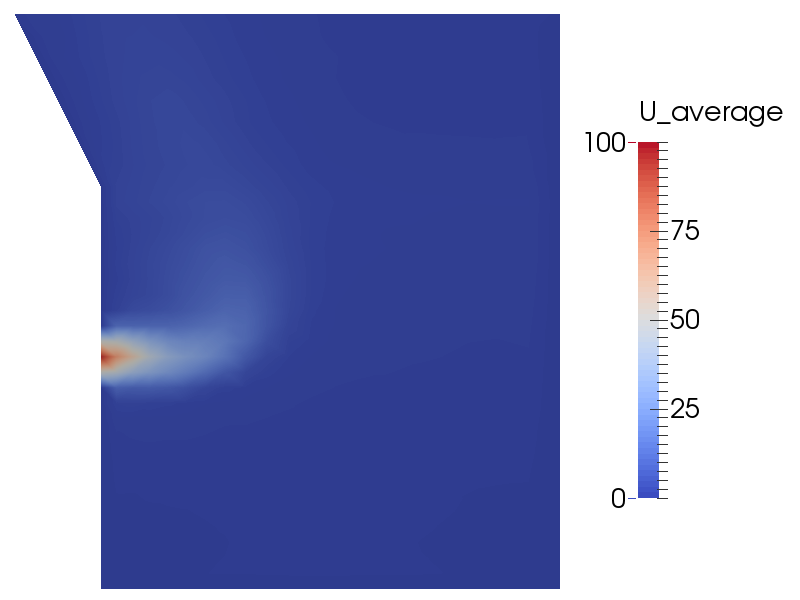
\includegraphics[width=.32\columnwidth]{images/227u_average_lf}
	  \label{fig:227u_average_lf}
  }
  \quad
    \subfloat[High friction, average velocity.]
    {
	  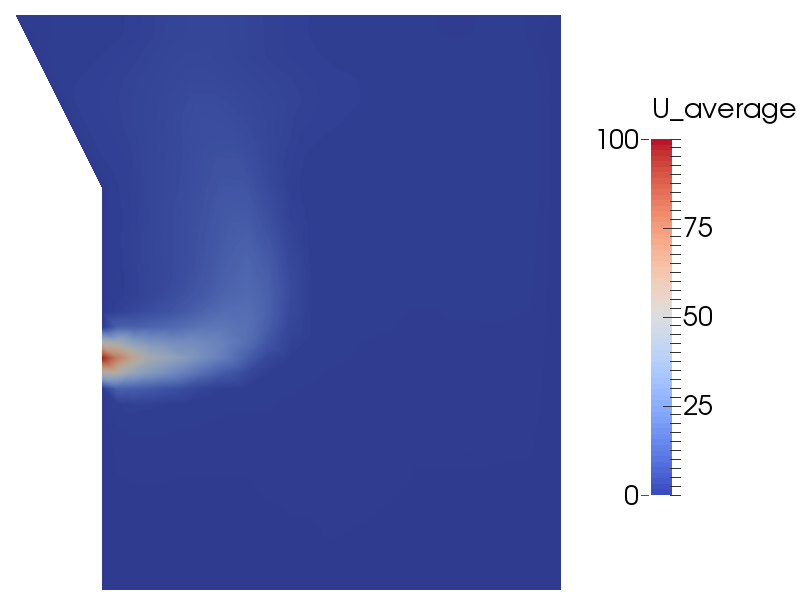
\includegraphics[width=.32\columnwidth]{images/226u_average_hf}
	  \label{fig:226u_average_hf}
  }
  \quad
    \subfloat[High friction, average velocity.]
    {
	  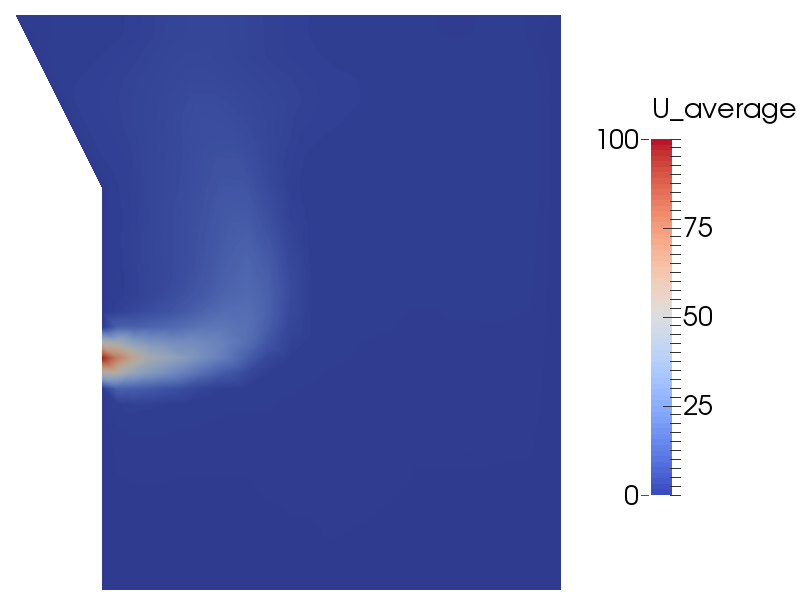
\includegraphics[width=.32\columnwidth]{images/226u_average_hf}
	  \label{fig:226u_average_hf}
  }
  \\
  \subfloat[Low friction, standard deviation velocity.]
  {
	  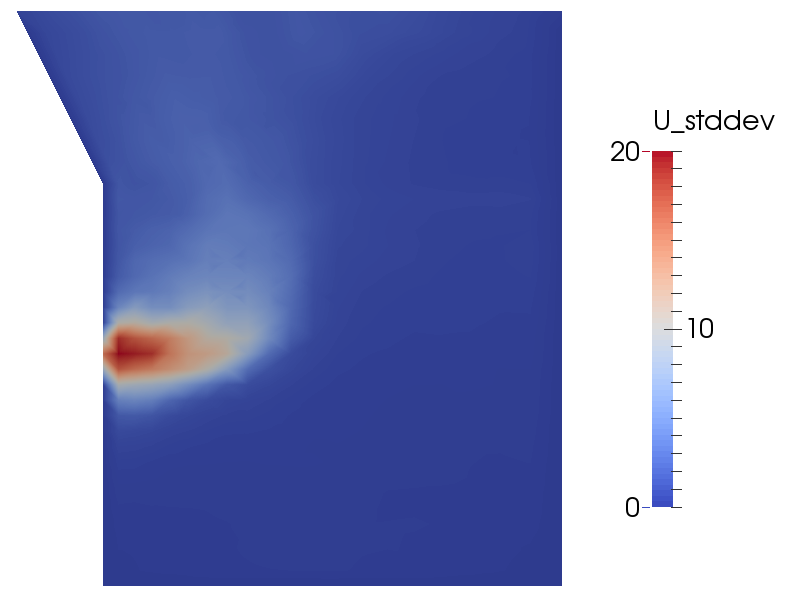
\includegraphics[width=.32\columnwidth]{images/229u_std_lf}
	  \label{fig:229u_std_lf}
  }
  \quad
    \subfloat[High friction, standard deviation velocity.]
    {
	  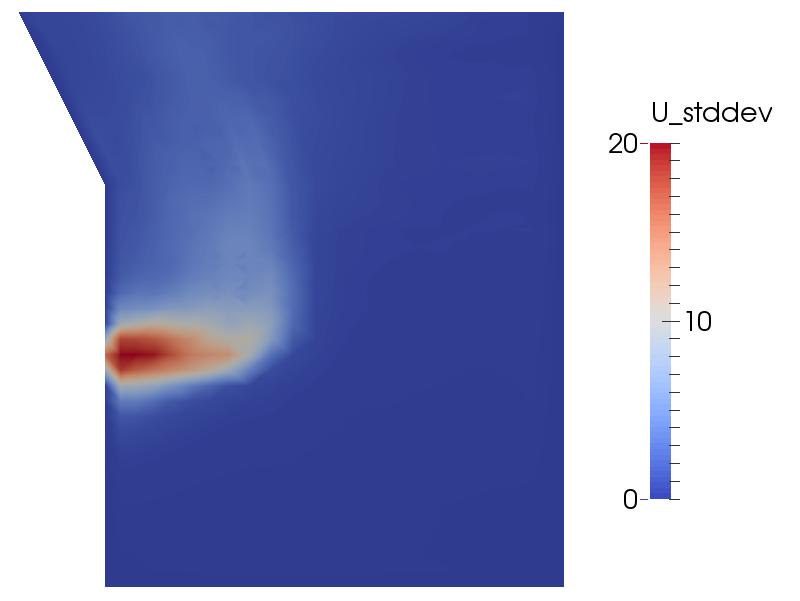
\includegraphics[width=.32\columnwidth]{images/228u_std_hf}
	  \label{fig:228u_std_hf}  }
  \\
  \caption{Fluid velocity with different sliding friction coefficient.}
  \label{fig:225racewayu}
\end{sidewaysfigure}
% \begin{sidewaysfigure}[htbp]
\centering 
  \subfloat[\acs{mus} = 0.1, \acs{mur} = 0.4, $v_{inlet}$ = 100 m/s .]
  {
	  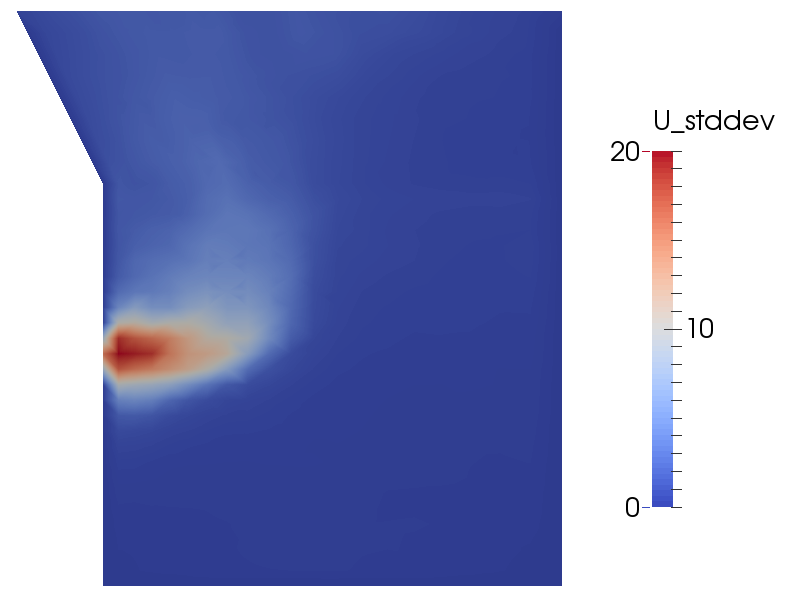
\includegraphics[width=.3\columnwidth]{images/229u_std_lf}
	  \label{fig:229u_std_lf}
  }
  \quad
    \subfloat[\acs{mus} = 0.5, \acs{mur} = 0.4, $v_{inlet}$ = 100 m/s .]
    {
	  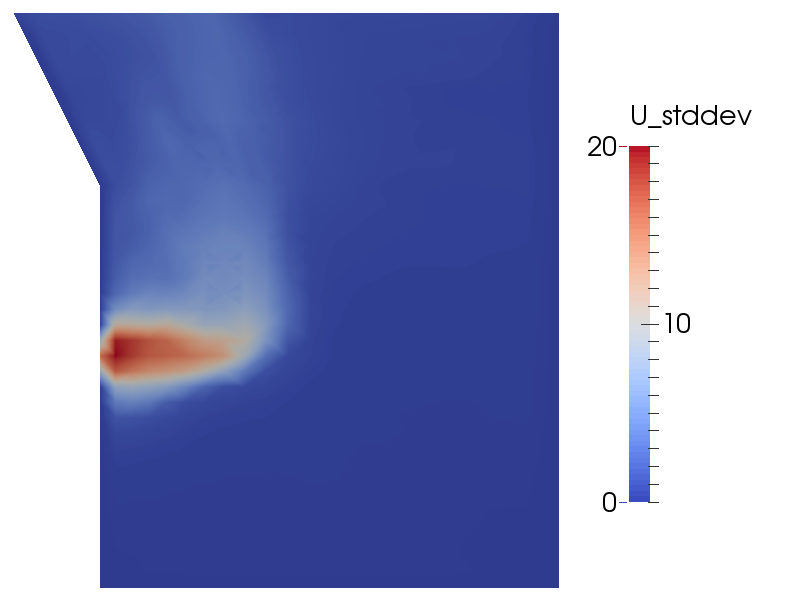
\includegraphics[width=.3\columnwidth]{images/245u_std_mf}
	  \label{fig:245u_std_mf}
  }
  \quad
    \subfloat[\acs{mus} = 0.9, \acs{mur} = 0.4, $v_{inlet}$ = 100 m/s .]
    {
	  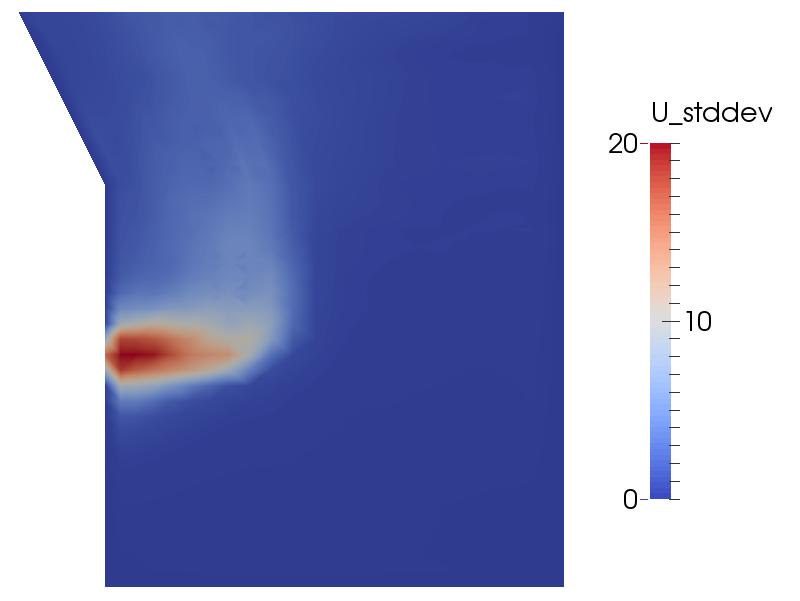
\includegraphics[width=.3\columnwidth]{images/228u_std_hf}
	  \label{fig:228u_std_hf}
  }
  \\
  \subfloat[\acs{mus} = 0.1, \acs{mur} = 0.4, $v_{inlet}$ = 200 m/s .]
  {
	  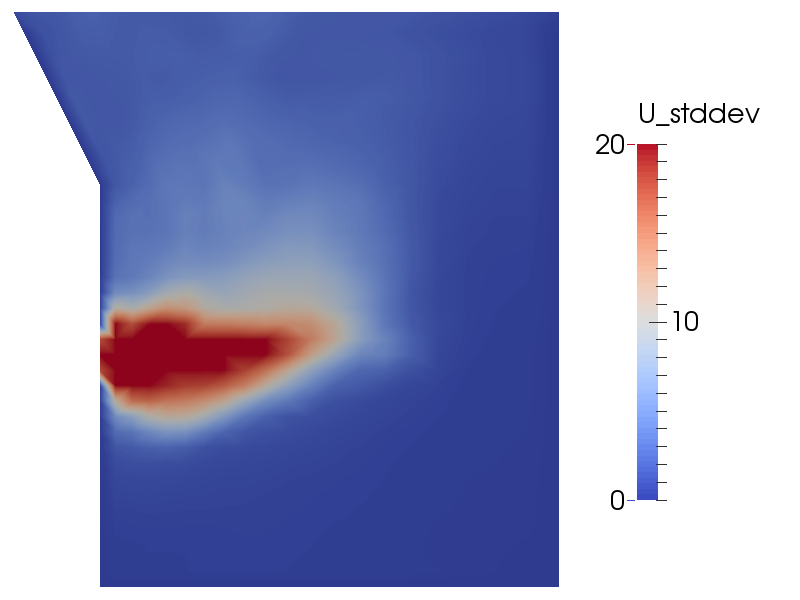
\includegraphics[width=.3\columnwidth]{images/244u_std_lfhv}
	  \label{fig:244u_std_lfhv}
  }
  \quad
    \subfloat[\acs{mus} = 0.9, \acs{mur} = 0.8, $v_{inlet}$ = 100 m/s .]
    {
	  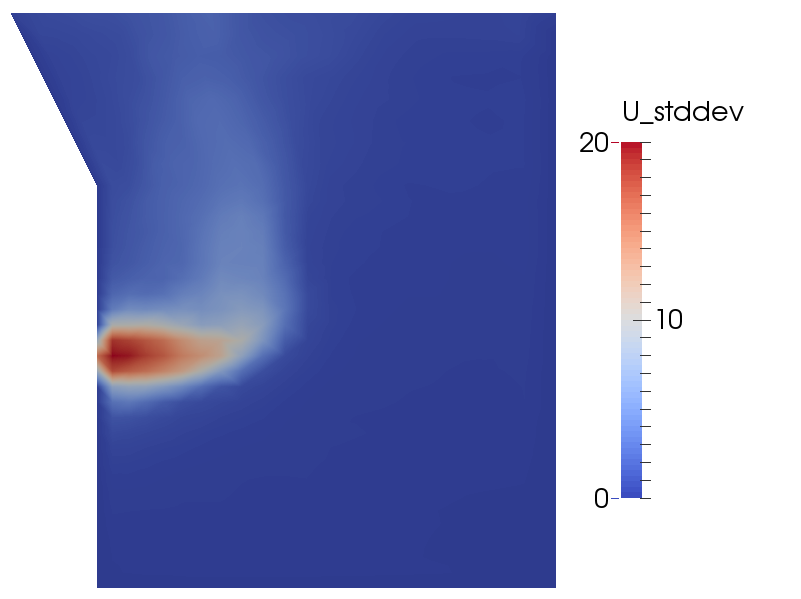
\includegraphics[width=.3\columnwidth]{images/243u_std_hfhr}
	  \label{fig:243u_std_hfhr}  }
  \\
  \caption{Standard deviation fluid velocity with different sliding friction
  coefficient.}
  \label{fig:258racewayustd}
\end{sidewaysfigure}
% \begin{sidewaysfigure}[htbp]
\centering 
  \subfloat[Low friction, average velocity.]
  {
	  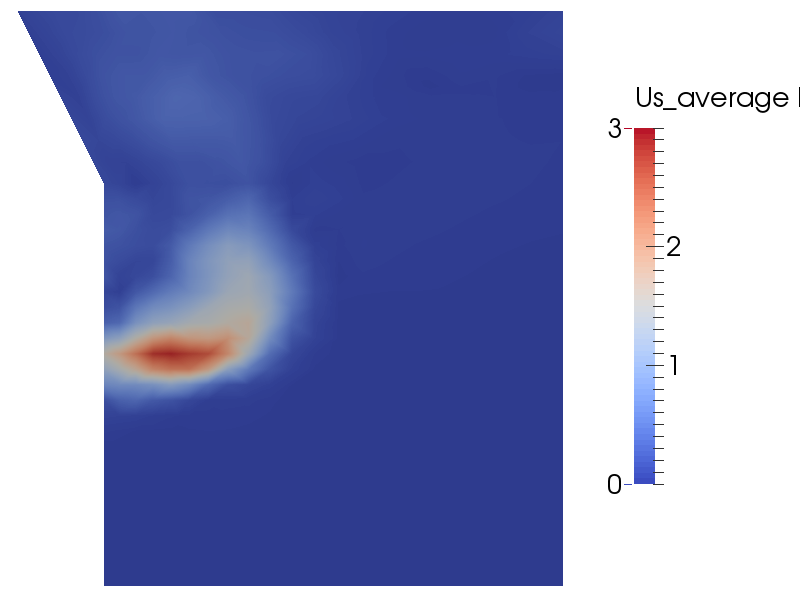
\includegraphics[width=.32\columnwidth]{images/231us_average_lf}
	  \label{fig:231us_average_lf}
  }
  \quad
    \subfloat[High friction, average velocity.]
    {
	  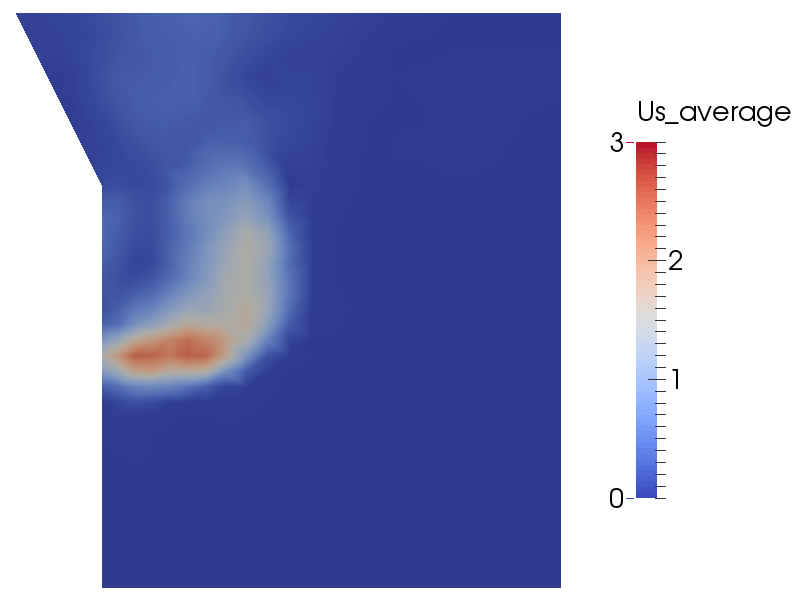
\includegraphics[width=.32\columnwidth]{images/230us_average_hf}
	  \label{fig:230us_average_hf}
  }
  \quad
    \subfloat[High friction, average velocity.]
    {
	  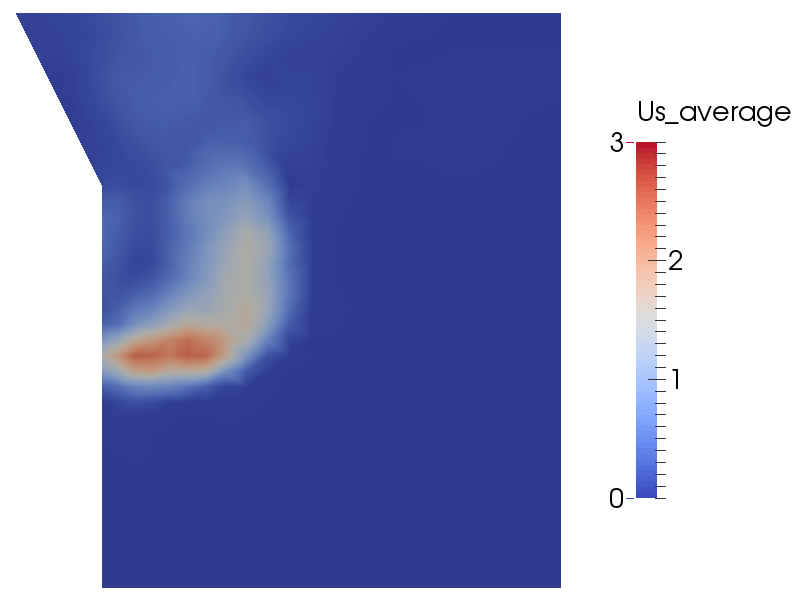
\includegraphics[width=.32\columnwidth]{images/230us_average_hf}
	  \label{fig:230us_average_hf}
  }
  \\
  \subfloat[Low friction, standard deviation velocity.]
  {
	  \includegraphics[width=.32\columnwidth]{images/233us_std_lf}
	  \label{fig:233us_std_lf}
  }
  \quad
    \subfloat[High friction, standard deviation velocity.]
    {
	  \includegraphics[width=.32\columnwidth]{images/232us_std_hf}
	  \label{fig:232us_std_hf}  }
  \\
  \caption{Particle velocity with different sliding friction coefficient.}
  \label{fig:238racewayus}
\end{sidewaysfigure}
% \begin{sidewaysfigure}[htbp]
\centering 
  \subfloat[\acs{mus} = 0.1, \acs{mur} = 0.4, $v_{inlet}$ = 100 m/s .]
  {
	  \includegraphics[width=.3\columnwidth]{images/233us_std_lf}
	  \label{fig:233us_std_lf}
  }
  \quad
    \subfloat[\acs{mus} = 0.5, \acs{mur} = 0.4, $v_{inlet}$ = 100 m/s .]
    {
	  \includegraphics[width=.3\columnwidth]{images/251us_std_mf}
	  \label{fig:251us_std_mf}
  }
  \quad
    \subfloat[\acs{mus} = 0.9, \acs{mur} = 0.4, $v_{inlet}$ = 100 m/s .]
    {
	  \includegraphics[width=.3\columnwidth]{images/232us_std_hf}
	  \label{fig:232us_std_hf}
  }
  \\
  \subfloat[\acs{mus} = 0.1, \acs{mur} = 0.4, $v_{inlet}$ = 200 m/s .]
  {
	  \includegraphics[width=.3\columnwidth]{images/250us_std_lfhv}
	  \label{fig:250us_std_lfhv}
  }
  \quad
    \subfloat[\acs{mus} = 0.9, \acs{mur} = 0.8, $v_{inlet}$ = 100 m/s .]
    {
	  \includegraphics[width=.3\columnwidth]{images/249us_std_hfhr}
	  \label{fig:249us_std_hfhr}  }
  \\
  \caption{Standard deviation particle velocity with different sliding friction
  coefficient.}
  \label{fig:259racewayusstd}
\end{sidewaysfigure}
% \begin{sidewaysfigure}[htbp]
\centering 
  \subfloat[Low velocity, average void fraction.]
  {
	  \includegraphics[width=.4\columnwidth]{images/235vf_average_lf}
	  \label{fig:235vf_average_lf}
  }
  \quad
    \subfloat[High friction, average void fraction.]
    {
	  \includegraphics[width=.4\columnwidth]{images/234vf_average_hf}
	  \label{fig:234vf_average_hf}
  }
  \\
  \subfloat[Low velocity, standard deviation void fraction.]
  {
	  \includegraphics[width=.4\columnwidth]{images/237vf_std_lf}
	  \label{fig:237vf_std_lf}
  }
  \quad
    \subfloat[High friction, standard deviation void fraction.]
    {
	  \includegraphics[width=.4\columnwidth]{images/236vf_std_hf}
	  \label{fig:236vf_std_hf}  }
  \\
  \caption{Void fraction with different sliding friction coefficient.}
  \label{fig:239racewayvf}
\end{sidewaysfigure}
% \begin{sidewaysfigure}[htbp]
\centering 
  \subfloat[Low friction, average void fraction.]
  {
	  \includegraphics[width=.3\columnwidth]{images/237vf_std_lf}
	  \label{fig:237vf_std_lf}
  }
  \quad
    \subfloat[High friction, average void fraction.]
    {
	  \includegraphics[width=.3\columnwidth]{images/257vf_std_mf}
	  \label{fig:257vf_std_mf}
  }
  \quad
    \subfloat[High friction, average void fraction.]
    {
	  \includegraphics[width=.3\columnwidth]{images/236vf_std_hf}
	  \label{fig:236vf_std_hf}
  }
  \\
  \subfloat[Low friction, standard deviation void fraction.]
  {
	  \includegraphics[width=.3\columnwidth]{images/256vf_std_lfhv}
	  \label{fig:256vf_std_lfhv}
  }
  \quad
    \subfloat[High friction, standard deviation void fraction.]
    {
	  \includegraphics[width=.3\columnwidth]{images/255vf_std_hfhr}
	  \label{fig:255vf_std_hfhr}  }
  \\
  \caption{Standard deviation void fraction with different sliding friction
  coefficient.}
  \label{fig:260racewayvfstd}
\end{sidewaysfigure}
% \begin{sidewaysfigure}[htbp]
\centering 
  \subfloat[Width [mm].]
  {
	  \includegraphics[width=.45\columnwidth]{images/261BoxLengthRaceway}
	  \label{fig:261BoxLengthRaceway}
  }
  \quad
    \subfloat[Height [mm].]
    {
	  \includegraphics[width=.45\columnwidth]{images/262BoxHeightRaceway}
	  \label{fig:262BoxHeightRaceway}
  }
  \\
    \subfloat[Height of the fast fluid area [mm].]
    {
	  \includegraphics[width=.45\columnwidth]{images/263BoxHeightRacewayChimney}
	  \label{fig:263BoxHeightRacewayChimney}
  }
  \quad
  \subfloat[Particles deleted during the simulations.]
  {
	  \includegraphics[width=.45\columnwidth]{images/264DeletedParticles}
	  \label{fig:264DeletedParticles}
  }
  \\
  \caption{Raceway results with different simulation parameters.}
  \label{fig:265racewaysummary}
\end{sidewaysfigure}


% Later, we trained a dedicated \acs{ANN} to evaluate the contribution of each of
% these parameters over the final results.